% --- ARCHIVO: Cap4_Reaccion_Reposicion/reaccion_reposicion.tex ---

\chapter{Reacción del Operador y Reposición del Suministro (Fase 4)}
\label{cap:reaccion_reposicion}

\section{Gestión de emergencia de Red Eléctrica: aplicación de los Procedimientos de Operación P.O.~1.1 y P.O.~1.6}
\label{sec:gestion_emergencia}

\lettrine[lines=3, lhang=0.1]{T}{ras} la consumación del \textit{Cero de Tensión} absoluto a las 12:33:30~CEST,
el sistema eléctrico peninsular transitó de una crisis dinámica incontrolable
a una fase de gestión de emergencia y reposición estructural. La magnitud del
colapso ---pérdida de más de 15~GW y desconexión total del sistema síncrono
continental--- obligó al Operador del Sistema (REE) a abandonar las lógicas
de operación en régimen permanente dictadas por el Procedimiento de Operación
P.O.~1.1 para activar los protocolos de emergencia previstos en el
\textit{Procedimiento de Operación
1.6}\textsuperscript{\ref{anexo:po16}} (P.O.~1.6) \cite{entsoe2025}.

\begin{figure}[H]
\centering
\resizebox{\textwidth}{!}{%
\begin{tikzpicture}[
    node distance=0.5cm,
    fase/.style={rectangle, rounded corners=4pt, fill=blue!15, draw=blue!40,
                 minimum width=2.6cm, minimum height=1.2cm, align=center,
                 font=\small\bfseries},
    fase3/.style={fase, fill=orange!15, draw=orange!40},
    fase4/.style={fase, fill=red!12, draw=red!35},
    fase5/.style={fase, fill=teal!12, draw=teal!40},
    hora/.style={rectangle, rounded corners=2pt, draw=gray!40,
                 minimum width=2.6cm, minimum height=0.9cm, align=center,
                 font=\footnotesize, below=0.15cm},
    arr/.style={->, thick, gray!60}
]

\node[fase]  (f0) {\textbf{Fase 0}\\Inestabilidad\\de tensiones};
\node[hora, below=0.15cm of f0] (h0) {D\'ias previos y\\ma\~nana del 28A};

\node[fase,  right=0.5cm of f0]  (f1) {\textbf{Fase 1}\\Oscilaciones\\del sistema};
\node[hora, below=0.15cm of f1] (h1) {12:00 ---\\12:30 CEST};

\node[fase3, right=0.5cm of f1]  (f2) {\textbf{Fase 2}\\P\'erdidas de gen.\\por sobretensi\'on};
\node[hora, below=0.15cm of f2] (h2) {12:32:00 ---\\12:33:18 CEST};

\node[fase4, right=0.5cm of f2]  (f3) {\textbf{Fase 3}\\Colapso hasta\\cero de tensi\'on};
\node[hora, below=0.15cm of f3] (h3) {12:33:18 ---\\12:33:30 CEST};

\node[fase5, right=0.5cm of f3]  (f4) {\textbf{Fase 4}\\Reposici\'on\\del suministro};
\node[hora, below=0.15cm of f4] (h4) {12:33:30 CEST ---\\14:36 del 29A};

\draw[arr] (f0) -- (f1);
\draw[arr] (f1) -- (f2);
\draw[arr] (f2) -- (f3);
\draw[arr] (f3) -- (f4);

\end{tikzpicture}}
\caption[Cronograma oficial de las fases del colapso y la restauración.]{%
Cronograma oficial de las fases del colapso y la restauración según
el Comité de Análisis del Gobierno.
Fuente: Comité de Análisis del Gobierno \cite{gobierno2025}}
\label{fig:cronograma_fases}
\end{figure}

La figura~\ref{fig:cronograma_fases} sintetiza la secuencia de cinco fases
en la que el Comité de Análisis del Gobierno estructura cronológicamente
el incidente. La Fase~4, objeto de este capítulo, marca el inicio formal
de los protocolos de emergencia y la suspensión del funcionamiento ordinario
del mercado eléctrico.

El P.O.~1.1 establece los criterios de funcionamiento y seguridad para la
operación del sistema en régimen permanente, fundamentados en el cumplimiento
del Criterio $N-1$ y en el mantenimiento de las tensiones entre 380~kV y
435~kV en la red de transporte. La cascada del 28 de abril mostró las
limitaciones de la validación estática de estos criterios frente a
transitorios dinámicos ultrarrápidos en redes de baja inercia: los límites
de seguridad térmica y angular previstos fueron superados en una ventana
de once segundos, y los esquemas de defensa automáticos ---incluyendo el
deslastre de cargas por subfrecuencia (UFLS)--- resultaron contraproducentes.
En ese momento, REE asumió el control manual y centralizado de la red bajo
estado de \textit{Apagón} (\textit{Blackout state}, criterio OB3)
\cite{icai2025}.

\clearpage

La reacción institucional fue inmediata y coordinada en varios frentes
simultáneos. A las 12:34~CEST, REE contactó con su homólogo portugués (REN)
para confirmar que la totalidad de la red lusa se encontraba igualmente sin
tensión. Dos minutos después, Red Eléctrica notificó formalmente la
situación al resto de operadores europeos de transporte a través del
\textit{ENTSO-E Awareness System} (EAS), modificando el estado operativo
del bloque ibérico a ``Restauración''. Paralelamente, el Gobierno de España
emitió la declaración oficial de ``Crisis de Electricidad'' ante la Comisión
Europea, amparándose en el Reglamento (UE)~2019/941 por superación extrema
de los umbrales de pérdida de carga \cite{gobierno2025}.

Para garantizar que la restitución topológica de la red se realizara sin
interferencias comerciales, el despacho central aplicó la normativa de
emergencia de forma estricta. A las 12:44~CEST, REE y el Operador del
Mercado Ibérico de Energía (OMIE) suspendieron todas las actividades de
los mercados intradiarios y de servicios de ajuste. Esta suspensión otorgó
a Red Eléctrica autoridad plena para despachar a los generadores
exclusivamente bajo criterios de viabilidad técnica y termodinámica,
marginando el mecanismo habitual de \textit{Orden de Mérito} económico.

La estrategia técnica de recuperación se articuló mediante la activación del
P.O.~1.6 (Establecimiento de los planes de seguridad y reposición), que
dictaminó la fragmentación controlada de la Península Ibérica en siete áreas
operativas independientes ---Zona Sur, Tajo-Centro, Levante y otras---
durante la re-energización progresiva \cite{ree2025}.

\vspace{0.6cm}
\begin{figure}[H]
    \centering
    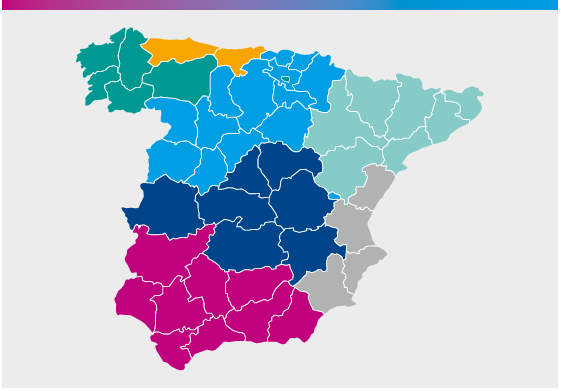
\includegraphics[width=0.85\textwidth]{figuras/islas_reposicion_entsoe.png}
    \vspace{0.2cm}
    \caption[Fragmentación topológica para la reposición del suministro (P.O. 1.6).]{%
    Fragmentación topológica de la península en siete islas eléctricas
    aisladas durante la reposición conforme al P.O.~1.6.
    Fuente: Informe Factual ENTSO-E / REE \cite{entsoe2025,ree2025}}
    \label{fig:islas_reposicion}
\end{figure}
\vspace{0.6cm}

La figura~\ref{fig:islas_reposicion} muestra la fragmentación topológica
aplicada en la reposición. Cada una de las siete islas eléctricas debía
estabilizarse individualmente en términos de tensión y frecuencia antes de
autorizarse su sincronización con las islas adyacentes, evitando así que
las inestabilidades locales se propagasen entre zonas durante la
recuperación.

La maniobra de emergencia combinó dos frentes simultáneos y complementarios.
Por un lado, una estrategia \textit{Top-Down} (de arriba hacia abajo)
solicitó apoyo externo urgente a Francia y a Marruecos con el fin de
disponer de una referencia de tensión y frecuencia externas estables desde
las que anclar las islas en formación. Por otro, una estrategia
\textit{Bottom-Up} (de abajo hacia arriba) activó el arranque autónomo de
las centrales hidroeléctricas internas de Galicia, Asturias y la cuenca del
Duero, únicas instalaciones capaces de arrancar sin tensión externa de red
\cite{nrel2025}.

\clearpage
% --------------------------------------------------------------
\section{Estrategia de \textit{Black Start}: priorización de centrales hidroeléctricas y ciclos combinados para el arranque autónomo}
\label{sec:black_start}
% --------------------------------------------------------------

Ante la confirmación del cero de tensión peninsular, REE y REN decretaron la
ejecución inmediata de la estrategia \textit{Bottom-Up} estipulada en sus
respectivos planes de reposición. Dado que la práctica totalidad del parque
generador ibérico estaba compuesto por \textit{Recursos Basados en
Inversores} (IBR) operando en modo \textit{grid-following}
---tecnológicamente incapaces de generar una onda de tensión sin una red
externa estable como referencia---, la supervivencia y el reinicio del
sistema recayeron de forma exclusiva sobre las máquinas síncronas
convencionales equipadas con capacidad de arranque autónomo
(\textit{Black Start})\textsuperscript{\ref{anexo:black_start}}.

\vspace{0.6cm}
\begin{figure}[H]
    \centering
    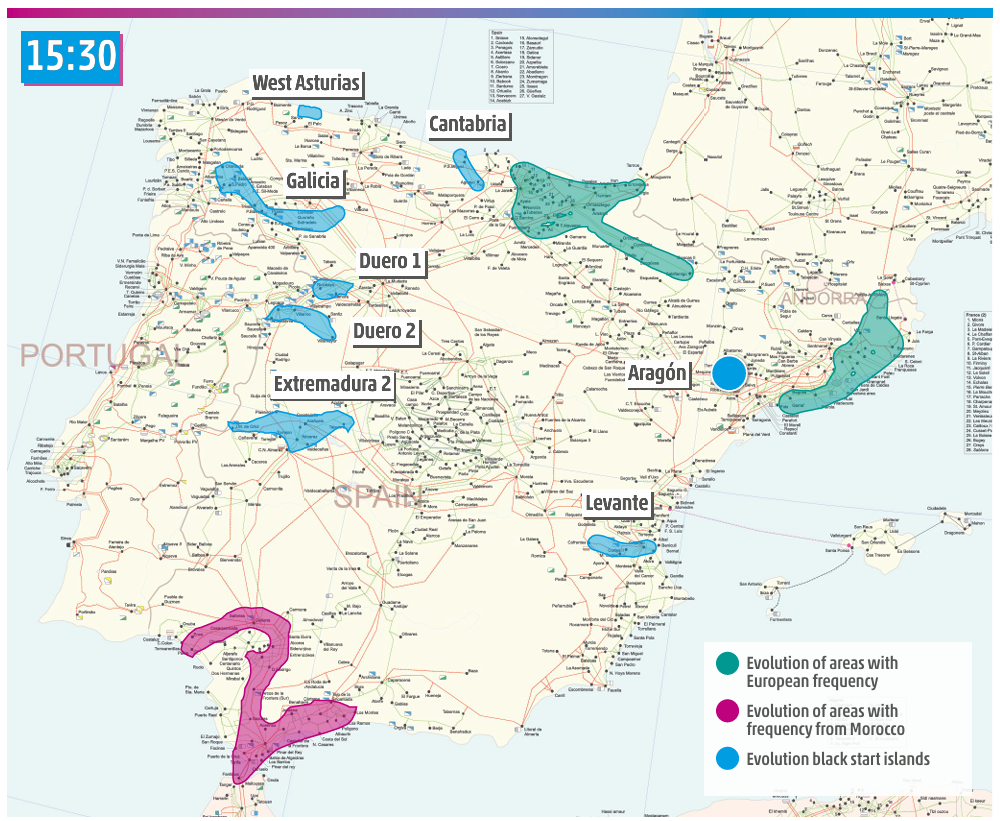
\includegraphics[width=0.9\textwidth]{figuras/estrategia_reenergizacion_dual.png}
    \vspace{0.2cm}
    \caption[Estrategia dual de re-energización (Top-Down y Bottom-Up).]{%
    Estrategia dual de re-energización aplicada por el Operador del
    Sistema: vía \textit{Top-Down} desde Francia y Marruecos y vía
    \textit{Bottom-Up} desde las centrales hidráulicas internas.
    Fuente: Informe Factual ENTSO-E / REE \cite{entsoe2025,ree2025}}
    \label{fig:estrategia_dual}
\end{figure}
\vspace{0.6cm}

La figura~\ref{fig:estrategia_dual} sintetiza las dos vías de re-energización
ejecutadas simultáneamente. La inyección de tensión de referencia desde
Francia y Marruecos proporcionó el ancla externa de las islas peninsulares,
mientras que el arranque autónomo de las centrales hidroeléctricas internas
permitió la formación de las primeras zonas energizadas en el norte
peninsular.

\clearpage

El primer eslabón de esta cadena de salvamento fueron las centrales
hidroeléctricas, tanto fluyentes como de bombeo. Al no depender de sistemas
térmicos auxiliares para iniciar su giro, estas instalaciones fueron las
primeras en ser despachadas para energizar tramos de red aislados y crear
las primeras ``islas eléctricas'' en torno a las cuencas del Duero, Galicia
y Asturias. Sin embargo, la operación de estos microsistemas mostró la
dificultad de operar con inercias mínimas: la energización de líneas en
vacío provocó transitorios capacitivos significativos que no permitieron
completar varios intentos de arranque \cite{entsoe2025}. Las islas formadas
en Cantabria y Levante no se sostuvieron y tuvieron que ser reiniciadas;
la central asignada a la isla de Madrid no logró estabilizar sus
parámetros tras varios intentos consecutivos; y el arranque autónomo en
Andalucía resultó infructuoso, lo que obligó a priorizar el apoyo externo
desde Marruecos como referencia de tensión para la zona sur.

\vspace{0.6cm}
\begin{figure}[H]
    \centering
    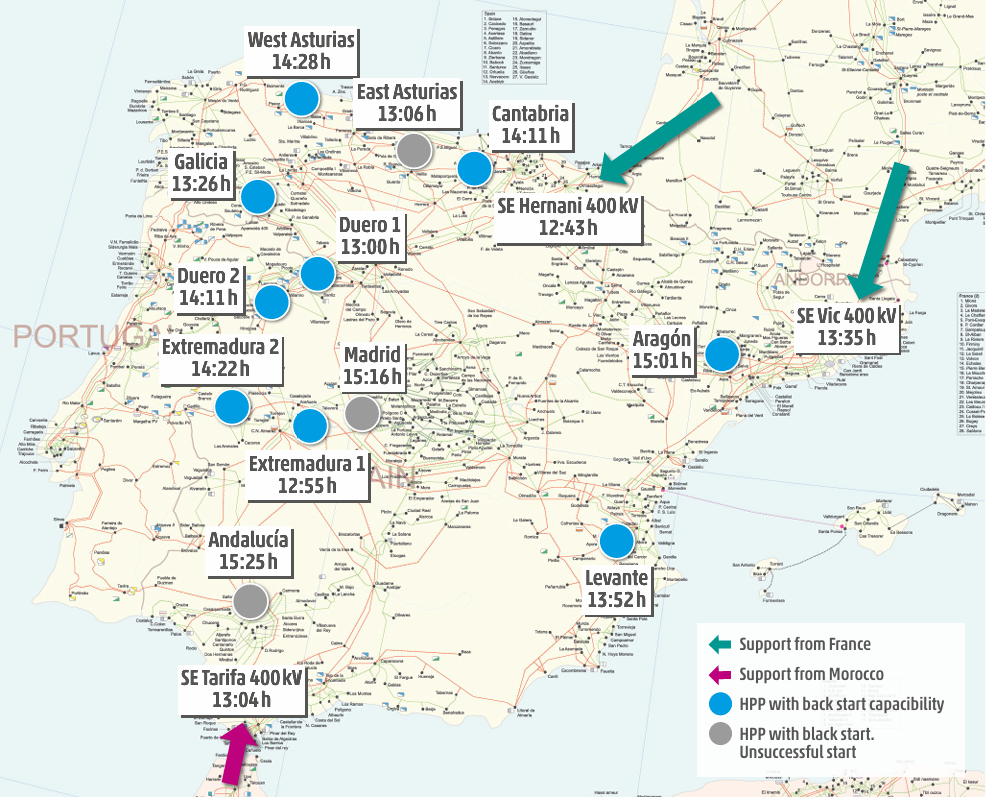
\includegraphics[width=0.85\textwidth]{figuras/black_start_hidroelectrico.png}
    \vspace{0.2cm}
    \caption[Despliegue temporal y eficacia del Black Start hidroeléctrico.]{%
    Despliegue temporal de los intentos de arranque autónomo
    hidroeléctrico durante la Fase~4. Los puntos grises corresponden a
    intentos no exitosos.
    Fuente: Informe Factual ENTSO-E / REE \cite{entsoe2025,ree2025}}
    \label{fig:black_start_hidro}
\end{figure}
\vspace{0.6cm}

La figura~\ref{fig:black_start_hidro} recoge el despliegue temporal de los
intentos de \textit{Black Start} hidroeléctrico. La elevada proporción de
intentos no exitosos (puntos grises) refleja la complejidad operativa de
energizar una red sin masa síncrona acoplada y obligó al Operador del
Sistema a readaptar progresivamente la topología de las islas a medida
que avanzaba la recuperación.

Una vez que las islas hidroeléctricas lograron estabilizar mínimamente sus
parámetros de tensión ($V$) y frecuencia ($f$), la estrategia viró hacia su
consolidación electromecánica mediante la integración de grandes masas
térmicas. La priorización inmediata fue el acoplamiento de las centrales de
Ciclo Combinado de Gas Natural (CCGT) y, progresivamente, la alimentación
de los servicios auxiliares de las centrales nucleares. La conexión de
estos grupos no perseguía inyectar volumen comercial de energía, sino actuar
como anclas dinámicas: aportaban la \textit{inercia del sistema} ($H$) y la
\textit{potencia de
cortocircuito}\textsuperscript{\ref{anexo:potencia_cortocircuito}}
($S_{sc}$) indispensables para dotar a las islas de la robustez necesaria
antes de autorizar la reconexión masiva de la demanda \cite{icai2025}.

En paralelo, el sistema eléctrico portugués ejecutó un esquema de
resiliencia análogo. REN fragmentó su recuperación apoyándose en dos pilares
de arranque autónomo: la central hidroeléctrica HPP~1-Centro y el ciclo
combinado CCGT~1-Norte. Aunque la hidroeléctrica lusa sufrió un disparo por
autoprotección en sus primeros compases al intentar conectar un
transformador de 220/60~kV, logró estabilizarse en el segundo intento. A
las 20:22~CEST, la sincronización de las islas portuguesas con las zonas
españolas ya acopladas a la frecuencia continental europea ---verificada
mediante \textit{relés de comprobación de
sincronismo}\textsuperscript{\ref{anexo:synchro_check}}
(\textit{synchro-check})--- marcó el hito que garantizó la viabilidad de
la reposición total de la Península Ibérica \cite{entsoe2025}.

\clearpage
% --------------------------------------------------------------
\section{Coordinación internacional: el papel de los Centros de Coordinación
Regional (RCC) y la sincronización con la red europea}
\label{sec:coordinacion_internacional}

La separación abrupta de la Península Ibérica del sistema síncrono de
Europa Continental trascendió las fronteras nacionales y exigió la
activación inmediata de los protocolos de soporte transfronterizo. En este
contexto, la arquitectura de seguridad europea ---vertebrada en torno a los
\textit{Centros de Coordinación
Regional}\textsuperscript{\ref{anexo:rcc}} (RCC)--- desempeñó un papel
dual: puso de manifiesto limitaciones analíticas de carácter preventivo y,
al mismo tiempo, resultó ser el pilar organizativo de la orquestación de la
recuperación y la resincronización \cite{entsoe2025}.

Durante las horas previas al incidente, el Centro de Coordinación Regional
responsable de la región de cálculo de capacidad del Suroeste de Europa
(SWE) ---Coreso--- había ejecutado de forma rutinaria sus tareas normativas
de planificación operativa (\textit{Outage Planning Coordination} y
\textit{Coordinated Security Analysis}). Todos los indicadores y modelos
de red común (CGM) arrojaron un estado seguro (``OK''), sin anticipar
congestiones ni violaciones del Criterio $N-1$ en los intercambios
fronterizos \cite{entsoe2025}.

\vspace{0.6cm}
\begin{figure}[H]
    \centering
    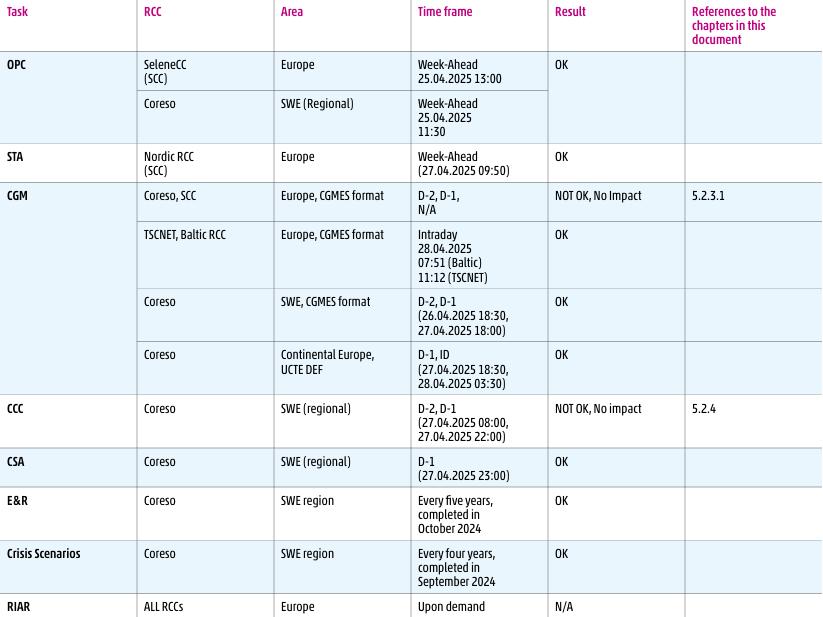
\includegraphics[width=0.85\textwidth]{figuras/validaciones_rcc_coreso.png}
    \vspace{0.2cm}
    \caption[Validaciones de seguridad estática previas al colapso.]{%
    Validaciones de seguridad estática realizadas por Coreso en las
    horas previas al colapso.
    Fuente: Informe Factual ENTSO-E \cite{entsoe2025}}
    \label{fig:validaciones_rcc}
\end{figure}
\vspace{0.6cm}

La figura~\ref{fig:validaciones_rcc} reproduce los resultados de las
validaciones de seguridad ejecutadas por Coreso en las horas previas al
incidente. La calificación del sistema como seguro en los análisis $N-1$
constata una limitación estructural del sistema europeo de monitorización:
las herramientas de los RCC evalúan la seguridad mediante flujos de carga
estáticos en régimen permanente, sin capacidad para anticipar fenómenos de
inestabilidad de tensión o dinámicas ultrarrápidas asociadas a la baja
inercia. En consecuencia, a través del \textit{ENTSO-E Awareness System}
(EAS), el bloque ibérico se mantuvo etiquetado bajo estado operativo
``Normal'' hasta el instante mismo del colapso ---tal como se analizó en
la sección~\ref{sec:eas_entsoe} (p.~\pageref{sec:eas_entsoe})--- privando
a los operadores vecinos de cualquier señal de alerta previa
\cite{mitceepr2025}.

\clearpage
Una vez consumado el cero de tensión, la jerarquía de mando europea se
activó a través de los Monitores del Área Síncrona (SAM), operados
conjuntamente por Swissgrid y Amprion. Entre las 12:49 y las 12:54~CEST,
estos centros confirmaron formalmente la situación de Emergencia y
establecieron una estructura de mando unificada para la restauración: Red
Eléctrica (REE) fue designada líder de frecuencia para la isla ibérica
desconectada, Swissgrid asumió el liderazgo para mantener estable el resto
del continente, y el operador francés (RTE) fue nombrado líder general de
resincronización (\textit{Resynchronisation Leader}) conforme a los
protocolos del plan de defensa europeo \cite{entsoe2025}.

Bajo este esquema de mando, la estrategia \textit{Top-Down} dependió
fundamentalmente de la potencia de cortocircuito aportada por los sistemas
vecinos indemnes. Por la frontera pirenaica, RTE desempeñó un papel
relevante: activó ofertas en su mecanismo de balance interno por hasta
4.500~MW para sostener la exportación hacia España, posibilitando la
energización progresiva de los corredores de 400~kV del norte y el este
peninsular \cite{entsoe2025}.

\vspace{0.6cm}
\begin{figure}[H]
    \centering
    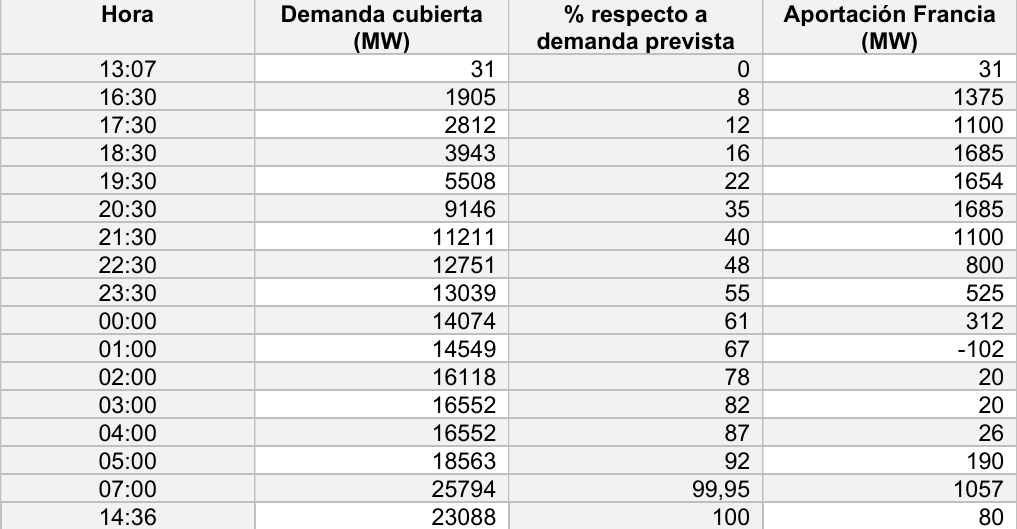
\includegraphics[width=0.85\textwidth]{figuras/evolucion_carga_repuesta_francia.png}
    \vspace{0.2cm}
    \caption[Evolución del soporte transfronterizo durante la reposición.]{%
    Evolución del soporte transfronterizo desde Francia durante la
    reposición.
    Fuente: Comité de Análisis del Gobierno \cite{gobierno2025}}
    \label{fig:evolucion_carga_francia}
\end{figure}
\vspace{0.6cm}

La figura~\ref{fig:evolucion_carga_francia} recoge la evolución del soporte
transfronterizo durante la reposición. Las inyecciones de potencia desde
Francia sostuvieron la estabilidad de tensión durante la re-energización
de los corredores norte y este de la península, antes de que los grupos
síncronos internos se acoplaran en cantidad suficiente.

Simultáneamente, en la frontera sur, la interconexión con Marruecos operada
por ONEE se convirtió en el ancla electromecánica de Andalucía. A las
13:04~CEST se habilitó el flujo de soporte a través de la línea de corriente
alterna Puerto de la Cruz--Mellousa, inyectando cerca de 900~MW y aportando
la referencia de tensión necesaria para energizar el sur peninsular, donde
los intentos de \textit{Black Start} hidroeléctrico no habían resultado
exitosos \cite{entsoe2025}.

\vspace{0.6cm}
\begin{figure}[H]
    \centering
    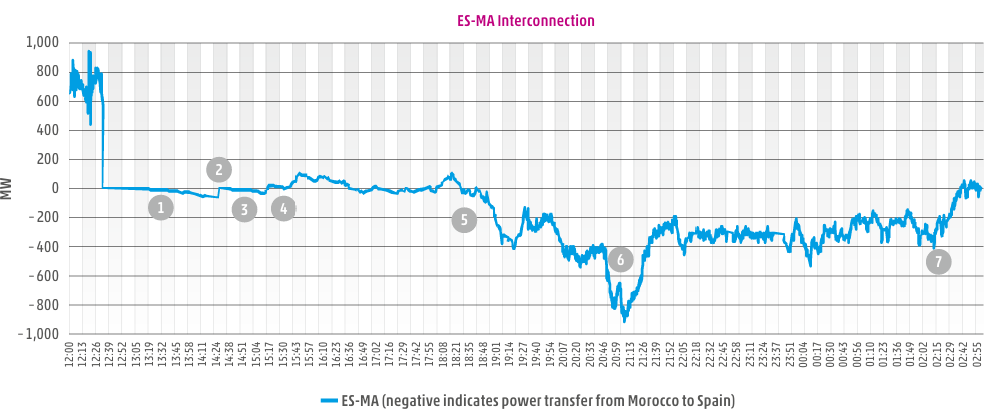
\includegraphics[width=0.85\textwidth]{figuras/intercambio_marruecos_topdown.png}
    \vspace{0.2cm}
    \caption[Inyección de potencia para el soporte Top-Down desde la frontera sur.]{%
    Inyección de potencia para el soporte \textit{Top-Down} desde la
    frontera sur (interconexión con ONEE).
    Fuente: Informe Factual ENTSO-E / REE \cite{entsoe2025,ree2025}}
    \label{fig:intercambio_marruecos}
\end{figure}
\vspace{0.6cm}

La interconexión con ONEE, recogida en la
figura~\ref{fig:intercambio_marruecos}, resultó determinante para aportar
la potencia de cortocircuito necesaria para energizar Andalucía tras el
fracaso de los arranques autónomos internos en la zona sur.

La comunicación continua y estructurada entre REE, REN, RTE, ONEE y los
centros de coordinación ---a través del EAS y canales bilaterales
directos--- permitió alinear progresivamente la frecuencia y acoplar las
sucesivas islas eléctricas restauradas a lo largo de la tarde. El panel de
expertos de ENTSO-E reconoció posteriormente esta cooperación
internacional como un caso de coordinación efectiva entre operadores
europeos ante eventos de severidad máxima (OB3) \cite{entsoe2025}.

% --------------------------------------------------------------
\section{Evolución del mix durante la reposición: gestión de la carga y
estabilización de la frecuencia}
\label{sec:evolucion_mix_reposicion}
% --------------------------------------------------------------

El éxito en la resincronización progresiva de la península exigió al
Operador del Sistema (REE) aplicar una discriminación tecnológica estricta
en el despacho de generación. A pesar de que los parques solares y eólicos
se encontraban físicamente intactos y con recurso primario disponible tras
el cero de tensión, su reconexión quedó restringida durante las primeras
fases críticas de la recuperación \cite{ree2025}.

Esta restricción obedeció a una limitación electromecánica fundamental: los
inversores operando en modo \textit{grid-following}, que equipaban a la
práctica totalidad del parque renovable español, carecen por diseño de la
capacidad de imponer una onda de tensión. Sus bucles de enganche de fase
(\textit{PLL}) necesitan leer previamente una red externa robusta y
estabilizada para inyectar corriente. En consecuencia, la responsabilidad
íntegra de la re-energización recayó sobre el acoplamiento secuencial de
las centrales síncronas: REE priorizó el arranque de los ciclos combinados
de gas natural (CCGT), las plantas de carbón remanentes y la recuperación
de los servicios auxiliares de las centrales nucleares \cite{ree2025}.

Estas máquinas térmicas no se conectaron inicialmente para satisfacer
demanda comercial, sino para conformar el ``andamiaje electromagnético''
del sistema: aportaban la potencia de cortocircuito ($S_{sc}$) necesaria
para energizar las líneas, la inercia del sistema ($H$) para absorber los
transitorios de conexión de cargas, y la capacidad de gestionar potencia
reactiva ($Q$) de forma continua mediante sus sistemas de excitación
\cite{icai2025}. Este rol de la generación síncrona como sustento
electromecánico de la recuperación constituye una constatación empírica
del análisis presentado en la sección~\ref{sec:justificacion_tecnica}
(p.~\pageref{sec:justificacion_tecnica}): su ausencia durante la operación
previa al colapso fue una de las condiciones operativas que el peritaje
identifica como facilitadoras del incidente.

\vspace{0.6cm}
\begin{figure}[H]
    \centering
    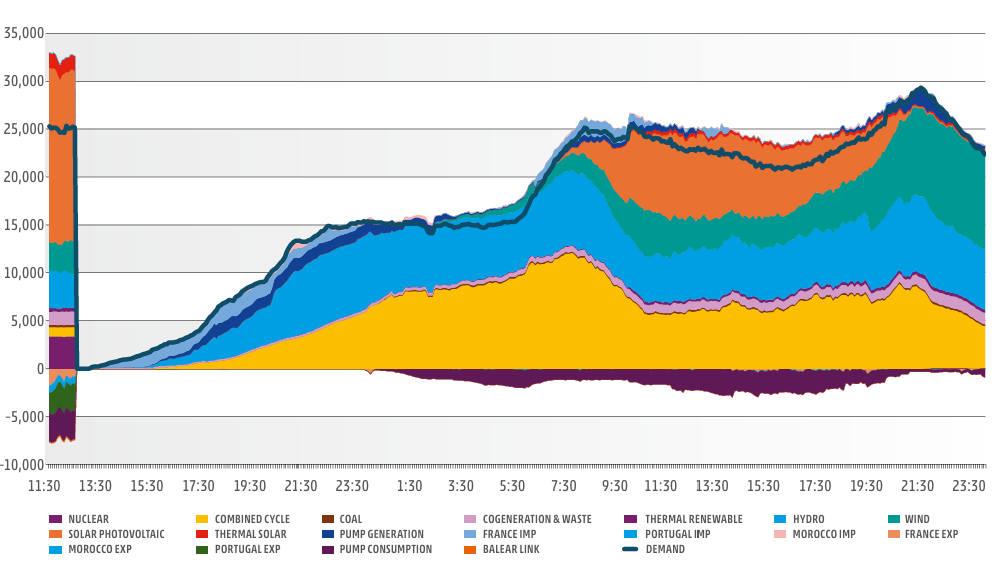
\includegraphics[width=0.85\textwidth]{figuras/evolucion_mix_reenergizacion.png}
    \vspace{0.2cm}
    \caption[Evolución del mix tecnológico durante la re-energización peninsular.]{%
    Evolución del mix tecnológico durante la re-energización peninsular.
    Fuente: Informe Factual ENTSO-E / REE \cite{entsoe2025,ree2025}}
    \label{fig:evolucion_mix_reenergizacion}
\end{figure}
\vspace{0.6cm}

La figura~\ref{fig:evolucion_mix_reenergizacion} muestra la evolución del
mix tecnológico durante la re-energización. Durante las primeras horas
críticas, el sistema se sostuvo exclusivamente mediante importaciones
transfronterizas y generación síncrona (térmica e hidráulica), sin la
participación del parque IBR en modo \textit{grid-following}. Esta
secuencia respondió a la necesidad de asegurar previamente la potencia de
cortocircuito y la inercia mínimas para la operación estable de los
inversores en modo seguidor de red.

\clearpage

Bajo este anclaje síncrono y el soporte exterior continuo, la carga se fue
reconectando en bloques discretos cuidadosamente calculados para evitar
que los transitorios hundieran nuevamente la frecuencia. El suministro se
reinició a las 13:07~CEST con la alimentación de los primeros 31~MW a
través de la subestación de Irún. La recuperación fue lenta durante las
primeras horas; al caer la noche, el acoplamiento sucesivo de islas
eléctricas aceleró el proceso. A las 23:32~CEST, con 21 grupos térmicos
ya sincronizados en la red peninsular, la demanda cubierta alcanzó los
13.039~MW, aproximadamente el 55~\% de la carga esperada
\cite{gobierno2025}.

Para consolidar la estabilización dinámica, a las 00:06~CEST del 29 de
abril REE reactivó el controlador maestro de la \textit{reserva de
restauración de frecuencia
automática}\textsuperscript{\ref{anexo:afrr}} (aFRR), devolviendo al
sistema ibérico su capacidad de regulación secundaria y de control
carga-frecuencia automatizado \cite{entsoe2025}. Este hito marcó el punto
a partir del cual el sistema dejó de depender exclusivamente del control
manual del operador.

Solo cuando la red alcanzó este estado de robustez inercial y tensional
suficientemente acreditada, el \textit{Centro de Control de Energías
Renovables}\textsuperscript{\ref{anexo:cecre}} (CECRE) autorizó la
reintegración paulatina de las tecnologías basadas en electrónica de
potencia. A partir de las 01:38~CEST se enviaron las primeras consignas
para permitir la inyección activa de parques eólicos y plantas de
cogeneración, liberándose las restricciones para la totalidad de las
instalaciones del régimen RCR (Renovables, Cogeneración y Residuos) a las
07:05~CEST. A esa misma hora, Red Eléctrica certificó la restitución del
99,95~\% del suministro eléctrico nacional, dando por concluida la crisis
a nivel de usuarios \cite{gobierno2025}.

\vspace{0.6cm}
\begin{figure}[H]
    \centering
    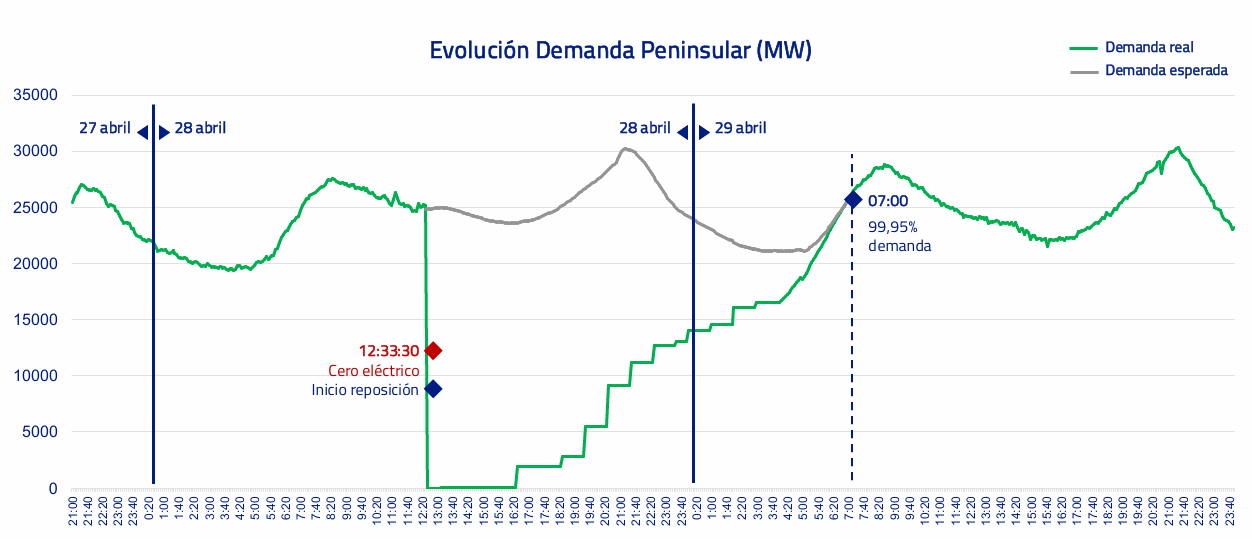
\includegraphics[width=0.85\textwidth]{figuras/recuperacion_demanda_peninsular.png}
    \vspace{0.2cm}
    \caption[Desplome y recuperación de la demanda eléctrica peninsular.]{%
    Desplome y recuperación de la demanda eléctrica peninsular durante
    las 19~horas posteriores al cero de tensión.
    Fuente: Presentación del Comité de Análisis del Gobierno
    \cite{gobierno2025}}
    \label{fig:recuperacion_demanda_peninsular}
\end{figure}
\vspace{0.6cm}

La figura~\ref{fig:recuperacion_demanda_peninsular} sintetiza el desplome
y la recuperación de la demanda peninsular. La reposición de los 25~GW
perdidos se completó tras casi 19~horas de maniobras ininterrumpidas, con
la conexión de carga escalonada para emparejarla con el acoplamiento
progresivo de las máquinas síncronas y evitar nuevos episodios de
subfrecuencia.